\begin{frame}{The dynamic connectome}

  \begin{columns}
    % 
    \begin{column}{.85\textwidth}

      
      \begin{figure}
        \hfill
        \includegraphics<1>[width=0.95\textwidth]{%
          figures/Loewenstein2015_Fig1A.png} %
      \end{figure}
      

    \end{column}
    % 
    \begin{column}{.15\textwidth}
      \minipage[c][0.65\textheight][s]{\columnwidth}
      \LARGE
      \vspace{2.3cm}
      Day 0

      \vspace{1.4cm}
      Day 4        
      \endminipage              
    \end{column}
  \end{columns}
  



  \pnote{
    
    - chronic two-photon imaging through\\
    a cranial window
    
    - auditory cortex in mice (expressing GFP\\
    in a subset of pyramidal neurons)

    Figure: 4 Days apart!

    - image spines from 8 neurons\\
    spine count almost constant!
    
    
  }

  
  \source{\cite{Loewenstein2015}}

  
\end{frame}


\begin{frame}{Robust nonrandom connectivity patterns}
  % 
  \begin{columns}
    % 
    \begin{column}{.45\textwidth}
      \minipage[c][0.75\textheight][s]{\columnwidth}
      
      \begin{figure}
        \centering
        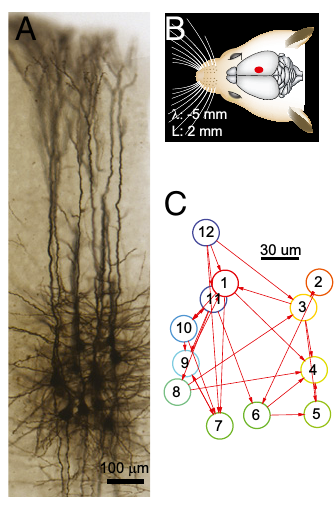
\includegraphics[width=\textwidth]{%
          figures/Perin2011_Fig1ABC.png} %
      \end{figure}
      

      
      \endminipage      
    \end{column}
    % 
    \begin{column}{.55\textwidth}
      \onslide<2->

      \vspace{-0.2cm}
      
      \begin{figure}
        \centering
        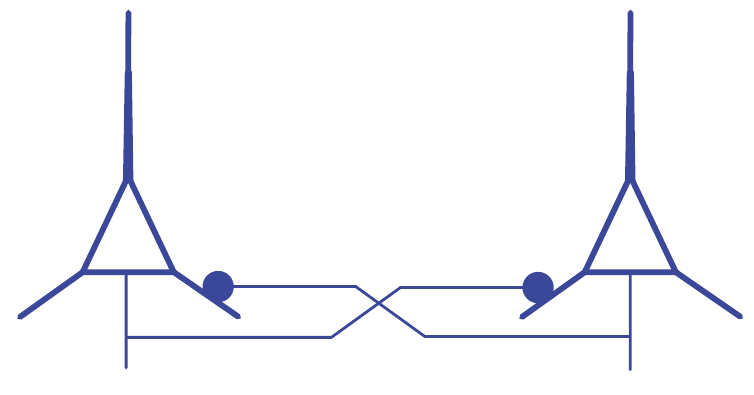
\includegraphics[width=0.525\textwidth]{%
          figures/two_neuron.png} %
      \end{figure}

      \vfill
      
      \onslide<3->
      \begin{figure}
        \centering
        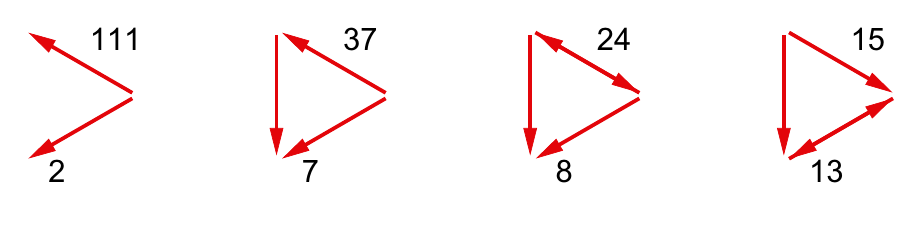
\includegraphics[width=\textwidth]{%
          figures/Perin2011_FigS2_custom.png} %
      \end{figure}

      \vfill
      
      \onslide<4->
      \begin{figure}
        \centering
        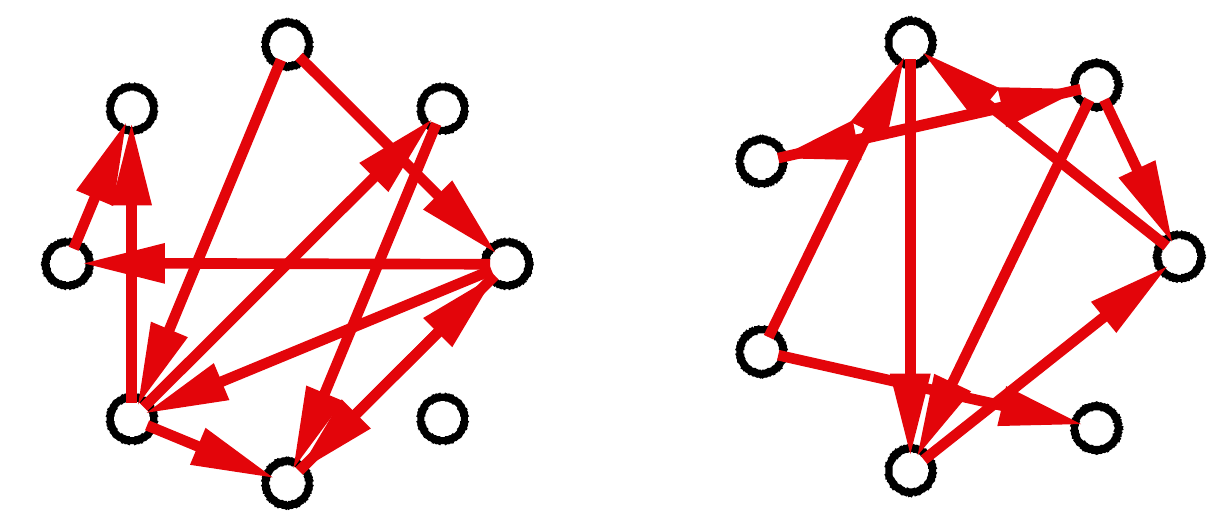
\includegraphics[width=0.7\textwidth]{%
          figures/clust_all.png} %
      \end{figure}
      
      \vfill

      
    \end{column}
  \end{columns}

  \source{\cite{Perin2011, Song2005, Markram1997, Miner2016, Gal2017,
      Vegue2017}}

  \pnote{
    
    These nonrandom structures are well established \\
    and have been reported both experimentally and  \\
    discussed theoretically, but it's interesting to \\
    think about these structures in the light of an \\
    everchanging and quickly rapidly connectome.
    
  }
  
\end{frame}